Since we are designing and conducting two user studies, other similar studies are of great interest to us. Through those existing works, we can learn more about the state of the art of study design and evaluation. \par \medskip

Obviously, the user study that guides our work the most is the one by \citet{gschwandtner2016visual}, as our aim is to build up on this work. This study compares six different techniques for the visualization of uncertainty in the temporal domain. To determine which technique works best for certain tasks, five different types of tasks were designed. The first type is about finding out how users interpret the different visualization techniques. In the second type of tasks the users are asked to read the boundaries of uncertainty intervals from the visualization. The third type is about determining the extent of an uncertainty interval. In the fourth type of tasks, the users have to gauge certain probabilities using the visualization and the last type of tasks asks the users for their opinion about the visualization. \par \medskip

\begin{figure}[H]
	\centering
	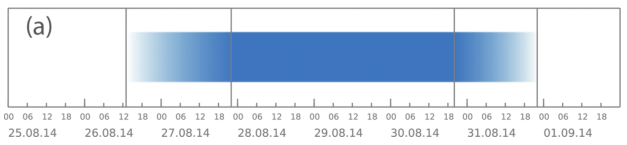
\includegraphics[width=0.85\textwidth]{figures/gradientplot.png}
	\caption{\textit{A gradient plot shows the certain parts of an interval as a solid color, while the uncertain parts are represented by a color gradient. \cite{gschwandtner2016visual}}}
	\label{fig:gradientplot}
\end{figure}

The actual study was conducted with 73 participants, which all were bachelor students in computer science. The students were recruited from a course in information design and visualization, which implies a certain knowledge about this topic. To automatically track relevant data, such as completion time and accuracy, during the study sessions, the EvalBench software library \cite{aigner2013evalbench} was utilized. This library was designed especially for the evaluation of visualization. To analyze the results Gschwandtner et al. ran an analysis of variance(ANOVA) for each task and subtask and backed up their results with a non-parametric Kruskal-Wallis test. Their analysis showed, that the technique \textit{ambiguation}, which can be seen in Figure \ref{fig:ambiguation}, works best for tasks in which the user has to judge the exact duration and bounds of an uncertainty interval. If the user has to determine certain probabilities within the uncertainty interval, \textit{gradient plots} (see Figure \ref{fig:gradientplot}) work best. \par \medskip

\begin{figure}[H]
	\centering
	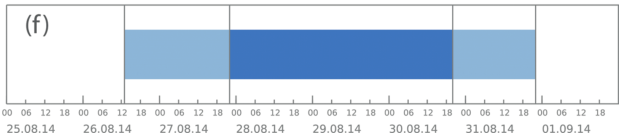
\includegraphics[width=0.85\textwidth]{figures/ambiguation.png}
	\caption{\textit{This technique is called ambiguation and shows the uncertain parts of a time interval in a lighter color than the certain part, which is represented by a solid color. \cite{gschwandtner2016visual}}}
	\label{fig:ambiguation}
\end{figure}

In our \textit{drawing study} our main focus lies on gauging how people think about certain situations and what kind of visualizations they associate with them. The goal is to find out what is intuitive for most people. These insights are valuable for the design of new visualizations, especially those aimed at non-expert users. \citet{maceachren2012visual} also tried to find out more about intuitive design of visualizations through user studies. Similar to us they conducted two separate user studies, which also have similar goals to ours. Their first study compares many different sets of symbols for the visualization of uncertainty, to find out which are most intuitive to people. Every set consists of three symbols, which encode high, medium and low uncertainty of 3 different kinds (accuracy, precision and trustworthiness), for 3 data domains (spatial, temporal and attribute). Some example sets can be seen in Figure \ref{fig:sets}. In total 102 symbol sets were rated by 31 undergraduate students for their intuitiveness on a scale from 1 to 7. After this first series of tests, the most unintuitive symbol sets were filtered out, which left 76 sets over. Those were again rated by 72 participants with a background in GIScience. \par \medskip

\begin{figure}[H]
	\centering
	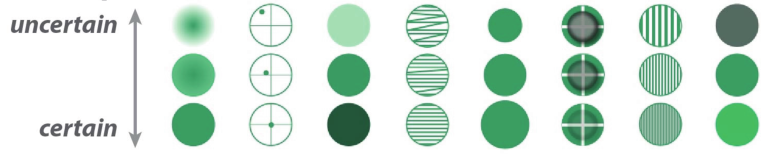
\includegraphics[width=0.75\textwidth]{figures/sets.png}
	\caption{\textit{Every column shows a set of three icons which represent high, medium or low uncertainty respectively. \cite{maceachren2012visual}}}
	\label{fig:sets}
\end{figure}

After this first study about intuitiveness, the 20 highest rated symbols for every combination of uncertainty type and data domain were compared in a second experiment. The goal of this subsequent study is to compare the selected visualizations' performance, so the combined results of both studies yield the best visualizations for a given task, which is intuitive and efficient at the same time. To compare the chosen symbols, two quadratic matrices with 9 symbols each were visualized side by side. The participants were asked to answer the question which of the two matrices featured a lower overall certainty, based on the presented symbols.  \par \medskip

\citet{walny2011visual} conducted a study with the goal of providing deeper insights into the way people think about and use visualizations to communicate their ideas. This study is relevant to our work, because it features a similar approach as our \textit{drawing study}. A total number of 69 researchers were observed using whiteboards during brainstorming, thinking, communication and similar actions. Whiteboards were chosen as a visualization medium, because they support a variety of thinking tasks, like personal and collaborative cognition, group meetings and planning. The results of the study feature interesting insights, such as different uses of emphasis techniques and the usage of ellipses as a focus and context technique. Our \textit{drawing study} aims to provide similar insights through a similar approach, by also observing users in their creation of visualizations and reviewing those drawings.\par \medskip

In another study of greater exploratory nature, \citet{walny2015exploratory} asked 22 participants (mostly computer science students) to sketch visualizations of a given dataset. The data was provided in a table format and was about appropriateness ratings of certain behavior in given situations. The student's task was to create visualizations to find interesting patterns in the data and articulate them in a post-sketching questionnaire. The results were analyzed through multiple coding passes, which showed that, even though 9 out of 22 participants claimed to have no experience in visualization, most of the sketched representations could be classified as known types.  As already stated, the study is of exploratory nature and therefore it does not answer many questions, but rather raises interesting questions and gives direction to future research.\par \medskip

There are user studies in the domain of information visualization which have the goal of determining if the visualization of a certain kind of information or a certain way of visualizing it is feasible or not. Our \textit{Evaluation Study} is one of those studies, since it aims to answer the question if it is advisable to visualize temporal uncertainties or if this information is not used in decision making and should therefore be omitted. Another similar study by \citet{xu2012user} is concerned with the feasibility of curved lines in graph layouts. In the study, graphs were visualized with either straight edges or three different kinds of curved edges and users were asked to perform certain tasks with a given graph. The completion time of those tasks and whether the final user decision was correct or incorrect, served as objective measures to rate the different graph layouts. Furthermore, the users were asked to give their personal opinion on which graphs they prefer and find visually more pleasing. An example graph in the three different layouts can be seen in Figure \ref{fig:graphs}. \par \medskip

\begin{figure}[H]
	\centering
	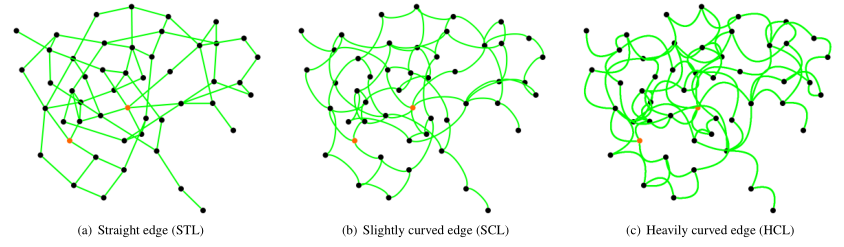
\includegraphics[width=0.85\textwidth]{figures/graphs.png}
	\caption{\textit{The same graph is drawn in three different curve layouts. (a) shows the graph drawn with straight edges, while (b) and (c) use slightly and heavily curved edges respectively. \cite{xu2012user}}}
	\label{fig:graphs}
\end{figure}

\citet{robertson2008effectiveness} conducted a study to get insights about the feasibility of animations in trend analysis visualizations. To answer the question if animation helps in the comprehension of visualized trends and in the completion of corresponding tasks, users were provided with one dynamic and two static data representations and asked to perform tasks with the presented data. One of the static representations showed the change within the data in traces of the changing data points, as can be seen in Figure \ref{fig:traces}. The tasks were either questions regarding the presented data or some kind of analysis task. During every study session, the completion time and the accuracy of the given answers were automatically recorded. To evaluate the results of the study, four hypothesis were formulated and tested for support within the resulting data. \par \medskip


\begin{figure}[H]
	\centering
	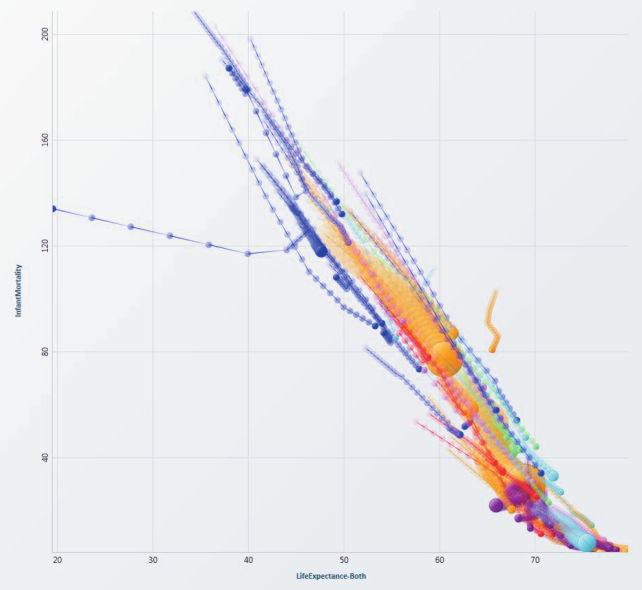
\includegraphics[width=0.45\textwidth]{figures/traces.png}
	\caption{\textit{The visualized data points are changing over time, which is statically represented by their traces. Traces are generated by drawing each point in its different stages over time and connecting these stages with lines. \cite{robertson2008effectiveness}}}
	\label{fig:traces}
\end{figure}